\documentclass{article}
\usepackage{graphicx}
\usepackage{lipsum}
\usepackage[T2A]{fontenc}
\usepackage[utf8]{inputenc}

\graphicspath{ {../Images/} }

\begin{document}
\begin{titlepage}
    \begin{center}
    $\newline$
    \vspace{3.3cm}
    
    {\LARGE\textbf{Лабораторна робота №2\\"Реалізація бітового потоку"}}
    \vspace{10cm}
    \begin{flushright}
        \textbf{Роботу виконав:}\\Климентьєв Максим \\3-го курсу\\групи ФІ-21
    \end{flushright}
    \end{center}
\end{titlepage}
\newpage

\tableofcontents 
\section{Особливості}
Якщо чесно --- \textbf{Чорна магія}, що воно взагалі працює для неповних бітів. Ніяк не допетрав як можна легко зробити зчитування декілька разів одного і того ж байту, з наборами бітів з різних сторін при цьому, щоб воно не ломало усе інше.
\section{Приклад}
    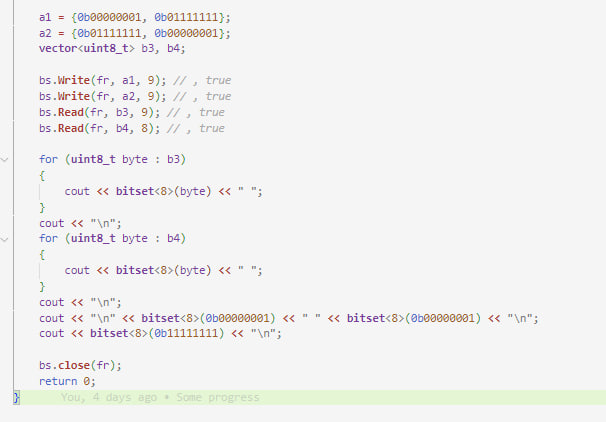
\includegraphics{example_code.jpg}
    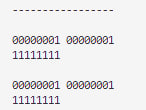
\includegraphics{example_result_and_expectations.jpg}

\end{document}